\documentclass[12pt,a4paper]{article}
\usepackage[utf8]{inputenc}
\usepackage[english]{babel}
\usepackage{amsmath}
\usepackage{amssymb}
\usepackage{amsthm}
\usepackage{graphicx}
\usepackage[hidelinks]{hyperref}
\usepackage{bookmark}
\usepackage{listings}
\usepackage{xcolor}
\usepackage{float}
\usepackage{booktabs}
\usepackage{geometry}
\usepackage[ruled,vlined]{algorithm2e}
\usepackage{tikz}
\usepackage{pgfplots}
\pgfplotsset{compat=1.18}
\usepackage{imakeidx}
\makeindex

% Page margins
\geometry{margin=1in}

% Theorem environments
\theoremstyle{definition}
\newtheorem{definition}{Definition}[section]
\newtheorem{theorem}{Theorem}[section]
\newtheorem{lemma}{Lemma}[section]

% Code listing style
\lstset{
    language=Python,
    basicstyle=\ttfamily\small,
    keywordstyle=\color{blue},
    commentstyle=\color{green!60!black},
    stringstyle=\color{red},
    numbers=left,
    numberstyle=\tiny\color{gray},
    frame=single,
    breaklines=true,
    captionpos=b
}

% Title information
\title{A Comprehensive Study of LaTeX Document Features\\
\large Sample Scientific Paper}
\author{Carlos Alberto Botina Carpio\\
University of American Samoa\\
\href{cbotina@americansamoa.edu}{cbotina@americansamoa.edu}}
\date{\today}

\begin{document}

\maketitle

\begin{abstract}
This document serves as a comprehensive showcase of various LaTeX features commonly used in scientific papers. We demonstrate mathematical notation, including inline and display formulas, complex equations, and mathematical symbols. Additionally, we present various document elements such as lists, tables, figures, algorithms, and code listings. The purpose of this paper is to serve as a reference template for creating well-formatted scientific documents using LaTeX.
\end{abstract}

\newpage
\tableofcontents
\newpage

% Include section files
\section{Introduction}

Scientific writing requires precise mathematical notation, clear presentation of data, and structured content organization. \LaTeX{}\index{LaTeX} provides powerful tools for achieving these goals. In this paper, we explore various \LaTeX{} features including:

\begin{itemize}
    \item Mathematical formulas\index{mathematical formulas} and equations\index{equations} (see Equation~\ref{eq:faraday})
    \item Structured lists\index{lists} (bulleted and numbered)
    \item Tables\index{tables} with professional formatting (see Table~\ref{tab:results})
    \item Figures\index{figures} and images\index{images} (see Figure~\ref{fig:example})
    \item Algorithms\index{algorithms} and pseudocode\index{pseudocode} (see Algorithm~\ref{alg:example})
    \item Code listings\index{code listings} (see Listing~\ref{lst:example})
    \item Theorems\index{theorems} and definitions\index{definitions}
\end{itemize}

Note: All cross-references work seamlessly across section files! You can reference tables, figures, equations, algorithms, etc. from any section file.


\section{Mathematical Formulas}\index{mathematical formulas|see{equations}}

\subsection{Inline Mathematics}

Mathematical expressions can be embedded within text, such as the famous Euler's formula: $e^{i\pi} + 1 = 0$, or Einstein's mass-energy equivalence $E = mc^2$. We can also express variables like $x$, $y$, and functions such as $f(x) = \int_{0}^{\infty} e^{-t^2} dt$.

\subsection{Display Mathematics}

For prominent equations, we use display mode:

\begin{equation}
    \nabla \times \mathbf{E} = -\frac{\partial \mathbf{B}}{\partial t}
    \label{eq:faraday}
\end{equation}

This is Faraday's law of electromagnetic induction. We can also express complex equations:

\begin{align}
    \frac{\partial u}{\partial t} + u \frac{\partial u}{\partial x} &= -\frac{1}{\rho}\frac{\partial p}{\partial x} + \nu \frac{\partial^2 u}{\partial x^2} \label{eq:navier-stokes-1} \\
    \frac{\partial \rho}{\partial t} + \frac{\partial (\rho u)}{\partial x} &= 0 \label{eq:continuity}
\end{align}

These equations represent the Navier-Stokes equations for fluid dynamics.

\subsection{Advanced Mathematical Notations}

We can express matrices:
\begin{equation}
    \mathbf{A} = \begin{pmatrix}
        a_{11} & a_{12} & \cdots & a_{1n} \\
        a_{21} & a_{22} & \cdots & a_{2n} \\
        \vdots & \vdots & \ddots & \vdots \\
        a_{m1} & a_{m2} & \cdots & a_{mn}
    \end{pmatrix}
\end{equation}

Or summations and products:
\begin{equation}
    \sum_{i=1}^{n} i = \frac{n(n+1)}{2}, \quad \prod_{i=1}^{n} i = n!
\end{equation}


\section{Lists and Structured Content}

\subsection{Bulleted Lists}

Itemized lists are useful for presenting key points:

\begin{itemize}
    \item First important point
    \item Second key observation
    \begin{itemize}
        \item Nested item at first level
        \item Another nested item
        \begin{itemize}
            \item Deeply nested item
        \end{itemize}
    \end{itemize}
    \item Final point
\end{itemize}

\subsection{Numbered Lists}

For sequential steps or ordered information:

\begin{enumerate}
    \item Initialize the system parameters
    \item Load the input data
    \item Process the data through the algorithm
    \item Evaluate the results
    \item Output the final solution
\end{enumerate}

\subsection{Descriptive Lists}

For definitions or explanations:

\begin{description}
    \item[Accuracy] The proportion of correct predictions among total predictions.
    \item[Precision] The proportion of true positives among all positive predictions.
    \item[Recall] The proportion of true positives that were correctly identified.
\end{description}


\section{Tables}

Tables\index{tables} are essential for presenting structured data. Table~\ref{tab:results} shows experimental results.

\begin{table}[H]
    \centering
    \caption{Experimental Results Comparison}
    \label{tab:results}
    \begin{tabular}{lccc}
        \toprule
        Method & Accuracy (\%) & Precision (\%) & F1-Score \\
        \midrule
        Baseline & 85.2 & 82.1 & 0.836 \\
        Method A & 89.7 & 87.3 & 0.885 \\
        Method B & 91.4 & 89.6 & 0.905 \\
        Method C & 93.8 & 92.1 & 0.929 \\
        \bottomrule
    \end{tabular}
\end{table}

Another example with more complex formatting:

\begin{table}[H]
    \centering
    \caption{Algorithm Performance Metrics}
    \label{tab:performance}
    \begin{tabular}{|l|r|r|r|}
        \hline
        \textbf{Algorithm} & \textbf{Time (s)} & \textbf{Memory (MB)} & \textbf{Iterations} \\
        \hline
        Gradient Descent & 12.34 & 256 & 1000 \\
        Newton's Method & 3.45 & 512 & 15 \\
        Conjugate Gradient & 8.76 & 384 & 150 \\
        \hline
    \end{tabular}
\end{table}


\section{Figures and Images}

Figures\index{figures} are crucial for visualizing results. Figure~\ref{fig:example} demonstrates how to include images\index{images} in a document.

\begin{figure}[H]
    \centering
    \includegraphics[width=0.7\textwidth]{img/img1.png}
    \caption{Example figure demonstrating data visualization. This could be a plot, diagram, or photograph relevant to the research.}
    \label{fig:example}
\end{figure}

Multiple figures can be arranged in subfigures:

\begin{figure}[H]
    \centering
    \begin{tabular}{cc}
        \includegraphics[width=0.45\textwidth]{img/img2.jpg} &
        \includegraphics[width=0.45\textwidth]{img/img3.jpg} \\
        (a) First subfigure & (b) Second subfigure
    \end{tabular}
    \caption{Multiple subfigures arranged side by side.}
    \label{fig:subfigures}
\end{figure}


\section{Graphs and Plots}

\LaTeX{} can create high-quality graphs\index{graphs} and plots\index{plots} using the \texttt{pgfplots}\index{pgfplots} package. Here are examples of different plot types commonly used in scientific papers.

\subsection{Line Plot}

Line plots are useful for showing trends over time or continuous data:

\begin{figure}[H]
    \centering
    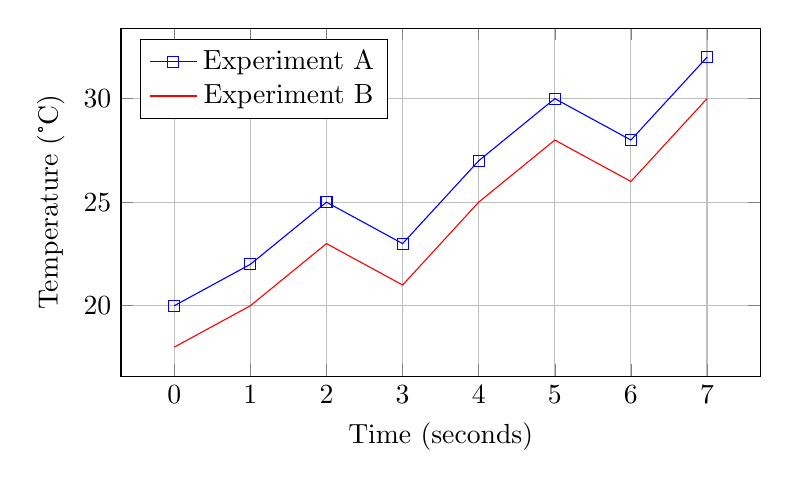
\begin{tikzpicture}
    \begin{axis}[
        xlabel={Time (seconds)},
        ylabel={Temperature (°C)},
        legend pos=north west,
        grid=major,
        width=0.8\textwidth,
        height=6cm
    ]
    \addplot[color=blue,mark=square] coordinates {
        (0,20) (1,22) (2,25) (3,23) (4,27) (5,30) (6,28) (7,32)
    };
    \addplot[color=red,mark=circle] coordinates {
        (0,18) (1,20) (2,23) (3,21) (4,25) (5,28) (6,26) (7,30)
    };
    \legend{Experiment A, Experiment B}
    \end{axis}
    \end{tikzpicture}
    \caption{Temperature measurements over time for two experiments.}
    \label{fig:lineplot}
\end{figure}

\subsection{Bar Chart}

Bar charts are ideal for comparing discrete categories:

\begin{figure}[H]
    \centering
    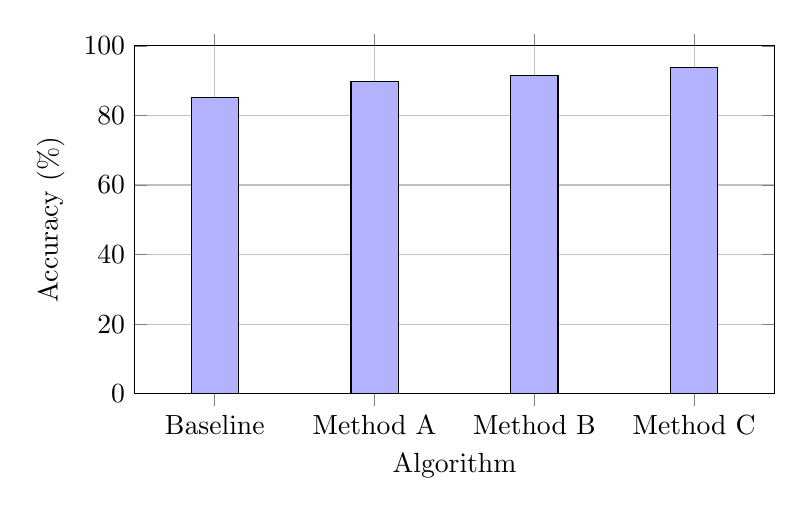
\begin{tikzpicture}
    \begin{axis}[
        ybar,
        bar width=0.6cm,
        xlabel={Algorithm},
        ylabel={Accuracy (\%)},
        xmin=-0.5,
        xmax=3.5,
        ymin=0,
        ymax=100,
        xtick=data,
        xticklabels={Baseline, Method A, Method B, Method C},
        grid=major,
        width=0.8\textwidth,
        height=6cm
    ]
    \addplot[fill=blue!30] coordinates {
        (0,85.2) (1,89.7) (2,91.4) (3,93.8)
    };
    \end{axis}
    \end{tikzpicture}
    \caption{Comparison of algorithm accuracy percentages.}
    \label{fig:barchart}
\end{figure}

\subsection{Scatter Plot}

Scatter plots show relationships between two variables:

\begin{figure}[H]
    \centering
    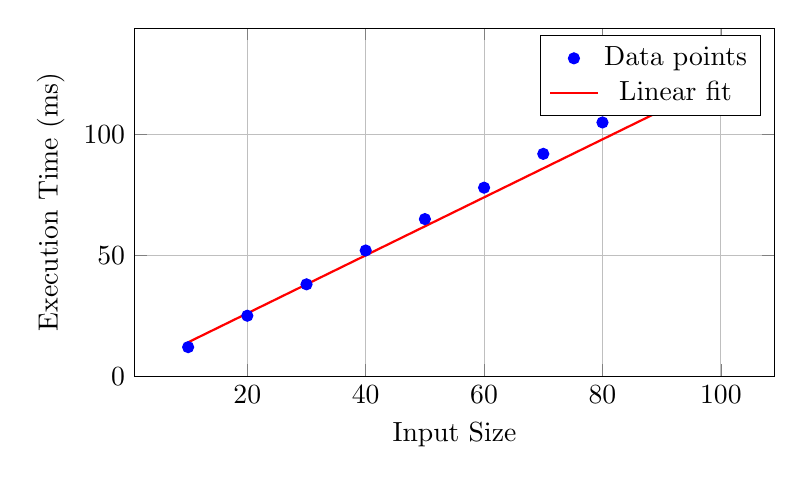
\begin{tikzpicture}
    \begin{axis}[
        xlabel={Input Size},
        ylabel={Execution Time (ms)},
        grid=major,
        width=0.8\textwidth,
        height=6cm
    ]
    \addplot[only marks,mark=*,mark size=2pt,color=blue] coordinates {
        (10,12) (20,25) (30,38) (40,52) (50,65) (60,78) (70,92) (80,105) (90,118) (100,132)
    };
    \addplot[color=red,thick,domain=10:100] {1.2*x + 2};
    \legend{Data points, Linear fit}
    \end{axis}
    \end{tikzpicture}
    \caption{Execution time versus input size with linear regression fit.}
    \label{fig:scatterplot}
\end{figure}

\subsection{Multiple Series Comparison}

Multiple data series can be compared in a single plot:

\begin{figure}[H]
    \centering
    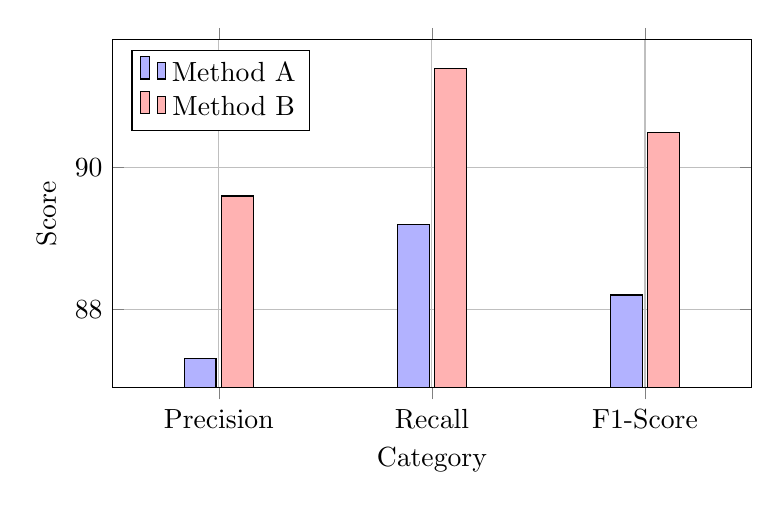
\begin{tikzpicture}
    \begin{axis}[
        ybar,
        bar width=0.4cm,
        xlabel={Category},
        ylabel={Score},
        xmin=-0.5,
        xmax=2.5,
        legend pos=north west,
        grid=major,
        width=0.8\textwidth,
        height=6cm,
        xtick=data,
        xticklabels={Precision, Recall, F1-Score}
    ]
    \addplot[fill=blue!30] coordinates {
        (0,87.3) (1,89.2) (2,88.2)
    };
    \addplot[fill=red!30] coordinates {
        (0,89.6) (1,91.4) (2,90.5)
    };
    \legend{Method A, Method B}
    \end{axis}
    \end{tikzpicture}
    \caption{Performance metrics comparison between two methods.}
    \label{fig:multibar}
\end{figure}


\section{Algorithms}

Algorithms\index{algorithms} are presented using pseudocode\index{pseudocode}. Algorithm~\ref{alg:example} shows a sample algorithm.

\begin{algorithm}[H]
    \caption{Example Algorithm for Optimization}
    \label{alg:example}
    \SetKwInOut{Input}{Input}
    \SetKwInOut{Output}{Output}
    \Input{Initial guess $x_0$, tolerance $\epsilon > 0$}
    \Output{Optimal solution $x^*$}
    Initialize $k \gets 0$\;
    $x \gets x_0$\;
    \While{$||\nabla f(x_k)|| > \epsilon$}{
        Compute search direction: $d_k \gets -\nabla f(x_k)$\;
        Compute step size: $\alpha_k \gets \arg\min_{\alpha} f(x_k + \alpha d_k)$\;
        Update: $x_{k+1} \gets x_k + \alpha_k d_k$\;
        $k \gets k + 1$\;
    }
    \Return{$x_k$}\;
\end{algorithm}


\section{Code Listings}

Code\index{code listings} can be included with syntax highlighting. Listing~\ref{lst:example} shows a Python\index{Python} example.

\begin{lstlisting}[caption={Example Python code for numerical computation}, label=lst:example]
import numpy as np
import matplotlib.pyplot as plt

def compute_gradient(x):
    """Compute the gradient of a function."""
    epsilon = 1e-8
    grad = np.zeros_like(x)
    for i in range(len(x)):
        x_plus = x.copy()
        x_plus[i] += epsilon
        grad[i] = (f(x_plus) - f(x)) / epsilon
    return grad

def gradient_descent(f, x0, learning_rate=0.01, max_iter=1000):
    """Perform gradient descent optimization."""
    x = x0.copy()
    for i in range(max_iter):
        grad = compute_gradient(x)
        x = x - learning_rate * grad
        if np.linalg.norm(grad) < 1e-6:
            break
    return x

# Example usage
x0 = np.array([1.0, 2.0])
result = gradient_descent(f, x0)
print(f"Optimal point: {result}")
\end{lstlisting}


\section{Theorems and Definitions}

\subsection{Definitions}

\begin{definition}[Convergence]
A sequence $\{x_n\}$ converges to a limit $L$ if for every $\epsilon > 0$, there exists a natural number $N$ such that for all $n > N$, we have $|x_n - L| < \epsilon$.
\end{definition}

\subsection{Theorems}

\begin{theorem}[Fundamental Theorem of Calculus]
If $f$ is continuous on $[a,b]$ and $F$ is an antiderivative of $f$ on $[a,b]$, then
\begin{equation}
    \int_a^b f(x) \, dx = F(b) - F(a)
\end{equation}
\end{theorem}

\begin{lemma}
For any positive real numbers $a$ and $b$, we have:
\begin{equation}
    \sqrt{ab} \leq \frac{a + b}{2}
\end{equation}
with equality if and only if $a = b$.
\end{lemma}


\section{Cross-References}

LaTeX provides powerful cross-referencing capabilities. We can reference:
\begin{itemize}
    \item Equations: see Equation~\ref{eq:faraday} or Equations~\ref{eq:navier-stokes-1} and~\ref{eq:continuity}
    \item Tables: Table~\ref{tab:results} and Table~\ref{tab:performance}
    \item Figures: Figure~\ref{fig:example} and Figure~\ref{fig:subfigures}
    \item Graphs: Figure~\ref{fig:lineplot}, Figure~\ref{fig:barchart}, Figure~\ref{fig:scatterplot}, and Figure~\ref{fig:multibar}
    \item Algorithms: Algorithm~\ref{alg:example}
    \item Code listings: Listing~\ref{lst:example}
    \item Sections: Section~\ref{sec:conclusion}
\end{itemize}


\section{Advanced Text Formatting}

Various text formatting options:

\begin{itemize}
    \item \textbf{Bold text}
    \item \textit{Italic text}
    \item \texttt{Monospace text}
    \item \textsc{Small caps}
    \item \underline{Underlined text}
    \item \emph{Emphasized text} (typically italic)
\end{itemize}

Special characters and symbols: \&, \%, \$, \#, \{, \}, \textbackslash.


\section{Conclusion}
\label{sec:conclusion}

This document demonstrates a comprehensive set of LaTeX features commonly used in scientific papers. We have covered mathematical notation, lists, tables, figures, algorithms, code listings, and various formatting options. This template can serve as a starting point for creating well-formatted scientific documents.

\section*{Acknowledgments}

We thank the LaTeX community for providing excellent documentation and tools for scientific typesetting.



% Bibliography and Index
\printindex

\bibliographystyle{ieeetr}
\bibliography{References}

\end{document}
